\section{Generieren}

Das Generieren der Statischen Punkt Wolke aus der die Galaxie abstrahiert wird
ist ein wichtiger Bestandteil des Gesamtprojektes, denn alles baut auf ihr auf.
Kurz: um Kräfte zwischen Sternen zu berechnen braucht man erstmal Sterne!

\subsection{Das Navarro-Frenk-White Profil}
Das Navarro-Frenk-White Profil (NFW-Profil) ist ein Profil das genutzt wird, um
die Räumilche Massen Verteilung von Sternen zu definieren. Es generiert für
einen Stern mit dem Abstand \( r \) zum Mittelpunkt der Galaxie eine
Warscheinlichkeit \( \rho \) welche definiert wie Warscheinlich es ist das der
Stern mit dem Abstand \( r \) generiert wird:

\begin{equation} \label{eq:NFW_profile}
  \rho_{NFW}(r) = \frac{ 1 }{ \sqrt{ 2 \pi } \cdot \sigma } \cdot
  \exp \left( \frac{ -\phi(r) }{ \sigma^{ 2 } } \right)
\end{equation}

\begin{equation*}
  \phi(r) = \frac{ 4\pi \cdot G \cdot f_{0} \cdot R_{s}^3 }{ r } \cdot
  ln{ \left( 1 + \frac{ r }{ R_{s} } \right) }
\end{equation*}

Es kann nun mithilfe der Random-Sampling Methode (\ref{subsec:random_sampling})
ermittelt werden, ob ein Stern beibehalten wird oder nicht.\\

\par Möchte man nun herausfinden wie weit ein Punkt mit der Koordinate \(
(x_{1}, x_{2}, x_{3}) \) vom Mittelpunkt des Raumes entfernt ist, kann der Satz
des Pythagoras (\ref{eq:pythagoras}) verwendet werden.

\begin{equation} \label{eq:pythagoras}
    r_{3} = \sqrt{x_{1}^{2} + x_{2}^{2} + x_{3}^{2} }
\end{equation}

Der Abstand \( r_{3} \) zum Mittelpunkt des Raumes kann nun in das NFW-Profil
(\ref{eq:NFW_profile}) gegeben werden um einen Wert \( s \) zu ermitteln welcher
beim Random Sampling verwendet wird:

\begin{equation}
\rho_{NFW}(r) = \dots = s
\end{equation}

Dieser Wert \( s \) stellt die Wahrscheinlichkeit dar, das ein Stern der
eine Entfernung \( r \) vom Mittelpunkt der Galaxie besitzt existiert.

Die Galaxie sieht aus der Ferne jetzt jedoch aus wie ein Würfel, da die aus \(
\rho_{NFW_{1}} \) resultierende Kurve abrupt endet. Dies kann gelöst werden,
indem statt \( \rho_{NFW_{1}}(r) \) folgendes gerechnet wird: \(
\rho_{NFW_{1}}(r) - \rho_{NFW_{1}}(r_{max}) = \rho_{NFW_{2}}(r)\)

\paragraph{Veranschaulichung:}~\\

\begin{center}
    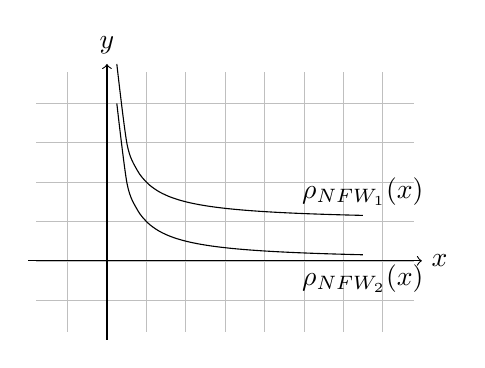
\begin{tikzpicture}
        \draw[very thin, color=lightgray, step=5mm] (-0.9, -0.9) grid (3.9, 2.4);
        \draw[->] (-1,0) -- (4,0) node[right] {$x$};
        \draw[->] (0,-1) -- (0,2.5) node[above] {$y$};
        \draw[scale=0.5, domain=0.25:6.5, smooth, variable=\x, black] plot ({\x},{(1/\x) + 1}) node[above] {$\rho_{NFW_{1}}(x)$};
        \draw[scale=0.5, domain=0.25:6.5, smooth, variable=\x, black] plot ({\x},{1/\x}) node[below] {$\rho_{NFW_{2}}(x)$};
    \end{tikzpicture}
\end{center}

Problematisch ist hierbei die Tatsache, dass aufgrund der Verschiebung die
Anzahl der Sterne die in Relation zu dem Bereich in dem sie generiert werden
sehr stark sinkt.

\subsection{Random Sampling} \label{subsec:random_sampling}

Um nun zu ermitteln ob ein Stern beibehalten wird oder nicht, wird die
Random-Sampling Methode verwendet.  Diese generiert in dem gegebenen Intervall,
welches zwischen der Minimalen und Maximalen Warscheinlichkeit welche aus dem
NFW-Profile entnommen werden, einen zufälligen Wert.

\begin{equation}\label{range:psi}
    \psi = [ \rho(r_{min}); \rho(r_{max}) ] 
\end{equation}

Sei \( s \) ein zufälliger Wert im Intervall \( \psi \).  Generiert man nun
einen zufälligen Wert \( r \) im Intervall \( \psi \), kann überprüft werden, ob \( s
> r \lor s < r \) gilt. Ist \( r
> s \), wird der Stern verworfen, ist \( r < s \) wird der Stern behalten.

\paragraph{Veranschaulichung:}~\\

\begin{center}
    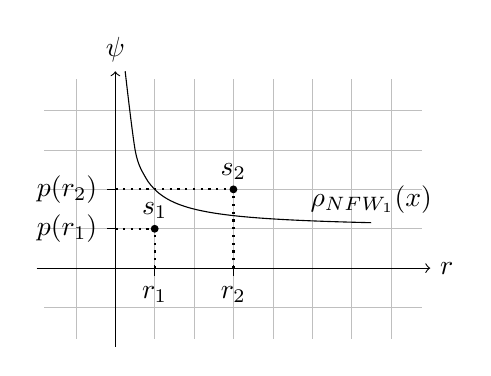
\begin{tikzpicture}
        % draw the background grid
        \draw[very thin, color=lightgray, step=5mm] (-0.9, -0.9) grid (3.9, 2.4);

        % draw the x-ticks
        \draw[xshift=0cm](0.5cm, 1pt) -- (0.5cm, -3pt) node[anchor=north] {$r_{1}$};
        \draw[xshift=0cm](1.5cm, 1pt) -- (1.5cm, -3pt) node[anchor=north] {$r_{2}$};

        % draw the y-ticks
        \draw[yshift=0cm](1pt, 0.5cm) -- (-3pt, 0.5cm) node[anchor=east] {$p(r_{1})$};
        \draw[yshift=0cm](1pt, 1.0cm) -- (-3pt, 1.0cm) node[anchor=east] {$p(r_{2})$};

        % draw the dotted lines connecting the point s_1
        \draw[thick, dotted] (0.5, 0) -- (0.5, 0.5);
        \draw[thick, dotted] (0, 0.5) -- (0.5, 0.5);

        % draw the dotted lines connecting the point s_2
        \draw[thick, dotted] (0, 1.0) -- (1.5, 1.0);
        \draw[thick, dotted] (1.5, 0) -- (1.5, 1.0);

        % draw the axes
        \draw[->] (-1,0) -- (4,0) node[right] {$r$};
        \draw[->] (0,-1) -- (0,2.5) node[above] {$\psi$};

        % draw the plot
        \draw[scale=0.5, domain=0.25:6.5, smooth, variable=\x, black]
            plot ({\x},{(1/\x) + 1}) node[above] {$\rho_{NFW_{1}}(x)$};

        % draw the points
        \fill (0.5, 0.5) circle (0.05) node[above] {$s_1$};
        \fill (1.5, 1) circle (0.05) node[above] {$s_2$};
    \end{tikzpicture}
\end{center}

In der obigen Abbildung ist zu sehen wir zwei zufällige Punkte \( s_1 \) und \(
s_2 \) generiert wurden.

Angenommen es wurde ein Stern generiert für den nach Formel
(\ref{eq:pythagoras}) gilt: \( r = \sqrt{x_{1}^{2} + x_{2}^{2} + x_{3}^{2}} =
\dots = r_1 \). Es wird dann ein Zufälliger Wert \( p(r_1) \) im in
(\ref{range:psi}) definierten Intervall generiert. Die folgenden zwei Fälle
können dann eintreten und werden wie in (\ref{cases:random_sampling})
beschrieben abgehandelt.

\kern-1em

\begin{equation}\label{cases:random_sampling}
\begin{cases}
s_1 \leq NFW(r_1) & \rightarrow \text{Stern wird beibehalten}\\
s_1 > NFW(r_1) & \rightarrow \text{Stern wird verworfen}
\end{cases} 
\end{equation}


\subsection{Lookup Tabellen}
Statt nun für jeden Stern die Distanz des jeweiligen Sternes \( r \) in das
NFW-Profil (\ref{eq:NFW_profile}) einzusetzen, kann das NFW-Profil im vorhinein
berechnet werden. Es wird dabei eine Tabelle erstellt in der die Entfernung des
Sternes zum Mittelpunkt der Galaxie der jeweiligen Wahrscheinlichkeit
zugeordnet wird:

\begin{center}
\begin{tabular} {l | l}
    \( r_1 \) & \( \rho_1 \) \\ \hline
    \( r_2 \) & \( \rho_2 \) \\ \hline
    \( r_3 \) & \( \rho_3 \) \\ \hline
    \( \dots \) & \( \dots \) \\ \hline
    \( r_n \quad n \in \mathbb{N} \) & \( \rho_n \quad n \in \mathbb{N} \) \\ \hline
\end{tabular}
\end{center}

Die Tabelle kann jedoch nicht so genaue Ergebnisse liefern wie das NFW-Profil,
sie kann jedoch so angepasst werden, dass sie in den Arbeitsspeicher passt und
somit das NFW-Profil so genau wie möglich widerspiegelt und das Generieren
stark verbessert. Mit genügend Arbeitsspeicher ist der Fehler dann auch
vernachlässigbar. Ein Kritischer Faktor, der beachtet werden muss wenn
Lookuptabellen genutzt werden, ist die Geschwindigkeit des jeweiligen
Speichermediums. Nutzt man z.B. Eine sehr langsame Festplatte kann es mehr
Sinne machen die jeweiligen Werte direkt zu berechnen. Dagegen ist eine
schnelle SSD (Solid-State-Drive) um einiges schneller.

\subsection{Beschleunigung der Generierung}
Es existieren mehrere Möglichkeiten die Generierung der Punkte zu verbessern.

Eine gute Möglichkeit ist die Nutzung von mehr Rechenleistung.  Bei der Nutzung
von \( n \) mal sovielen Rechen kernen ist das Generieren von Sternen \( n \)
mal schneller. Die Server des Server-Hosters Hetzner können dabei gut
verwendet werden: Es wird stündlich abgerechnet und 32 Kerne mit 128 GB RAM
kosten \( \approx \) 50ct/h was es ermöglicht für einen vergleichsweisen
Günstigen Preis, sehr viele Koordinaten zu generieren.

Die Ausgabe von jeder Potentiellen Koordinate in die Kommandozeile verlangsamt
die Generierung unglaublich stark, da der Rechner darauf wartet das die Ausgabe
fertig ist bevor er mit der nächsten Rechnung beginnt was zu einer relativ
starken Verlangsamung der Generierung führt.
